\chapter{Opis teoretyczny}
\label{cha:opis_teor}

\section{Gra}
\label{sec:gra}
Niniejsza praca skupia się na grach wieloosobowych, których szczególnym przypadkiem jest gra 3-osobowa \cite{Str01}. Model gry 3-osobowej pokazuje, że decyzję jednego z zawodników mają bezpośredni wpływ na zachowanie sąsiadów. W modelu gry N-osobowej decyzje graczy będą wpływać nie tylko na najbliższych sąsiadów, ale pośrednio także na decyzje innych graczy.
Omawiane tutaj gry są grami o niepełnej informacji, w tej pracy oznacza to grę, w której nie wszyscy uczestnicy znają prawdopodobieństwo określonych decyzji przeciwników. Prawdopodobieństwo gry przeciwników będzie szacowane na podstawie obserwacji historii ich zagrań.
Opisywane gry będą także grami ewolucyjnymi, gdzie gracze mają możliwość przewidywania i uczenia się na podstawie zachowań innych graczy.

\section{Model gry}
\label{sec:model}
Jak wcześniej wspomniano będą potrzebne dwa modele gier. Pierwszym z nich będzie model gry 3-osobowej (Rys. \ref{fig:model_niezal}). Graczy nazwiemy odpowiednio $G_0$, $G_1$, $G_2$ (gracz zerowy, pierwszy, drugi). Zachowanie każdego z nich jest opisane prawdopodobieństwem próby wejścia w koalicję z graczem o wyższym indeksie. To prawdopodobieństwo oznaczone jest jako $p_i$ ($i$ jest indeksem gracza), przy czym dla $G_2$ gracz o wyższym indeksie to $G_0$. Prawdopodobieństwo zagrania, w celu nawiązanie koalicji z graczem o niższym indeksie to $1 - p_i$. Analogicznie dla $G_0$ gracz o niższym indeksie to $G_2$. Ponieważ omawiana jest gra o niepełnej informacji żaden z zawodników nie ma dostępu do prawdopodobieństw innych graczy, lecz każdy ma dostęp do statystyki gry na którą składa się:
\begin{itemize}
\item $l_p$ liczba rozegranych w grze partii
\item $n_i$ ilość zagrań $G_i$ w celu zawiązania sojuszu z $G_{i+1}$, ilość zagrań $G_{i}$ aby nawiązać sojusz z $G_{i-1}$ wyraża się jako $l_p - n_i$
\end{itemize}
Model gry N-osobowe (Rys. \ref{fig:model_zal}) \cite{Fsmd} będzie opisany takimi samymi danymi jak model gry 3-osobowej. Różnicą między nimi będzie ustawienie graczy w okręgu, co w konsekwencji pokaże skutki decyzji wykraczające poza najbliższych sąsiadów, dla gier o liczbie graczy większej niż 3. Gra 3-osobowa jest szczególnym przypadkiem gry N-osobowej, w której konsekwencje zachowań jednego z naszych sąsiadów bezpośrednio wpływają na drugiego.
\begin{figure}
	\centering
	\begin{tabular}{c|c}
	\subfloat[3-osobowej \label{fig:model_niezal}]{ 
		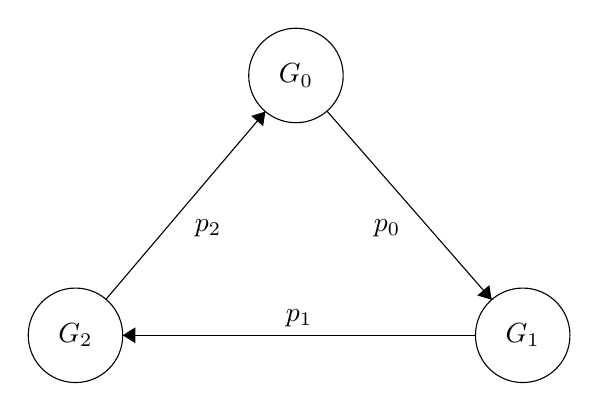
\begin{tikzpicture}[scale=0.2]
		\tikzstyle{every node}+=[inner sep=0pt]
		\draw [black] (40.6,-18.2) circle (3);
		\draw (40.6,-18.2) node {$G_0$};
		\draw [black] (55,-34.7) circle (3);
		\draw (55,-34.7) node {$G_1$};
		\draw [black] (26.6,-34.7) circle (3);
		\draw (26.6,-34.7) node {$G_2$};
		\draw [black] (42.57,-20.46) -- (53.03,-32.44);
		\fill [black] (53.03,-32.44) -- (52.88,-31.51) -- (52.12,-32.17);
		\draw (47.26,-27.9) node [left] {$p_0$};
		\draw [black] (52,-34.7) -- (29.6,-34.7);
		\fill [black] (29.6,-34.7) -- (30.4,-35.2) -- (30.4,-34.2);
		\draw (40.8,-34.2) node [above] {$p_1$};
		\draw [black] (28.54,-32.41) -- (38.66,-20.49);
		\fill [black] (38.66,-20.49) -- (37.76,-20.77) -- (38.52,-21.42);
		\draw (34.15,-27.89) node [right] {$p_2$};
		\end{tikzpicture}
	} &
	\subfloat[N-osobowej \label{fig:model_zal}]{  
		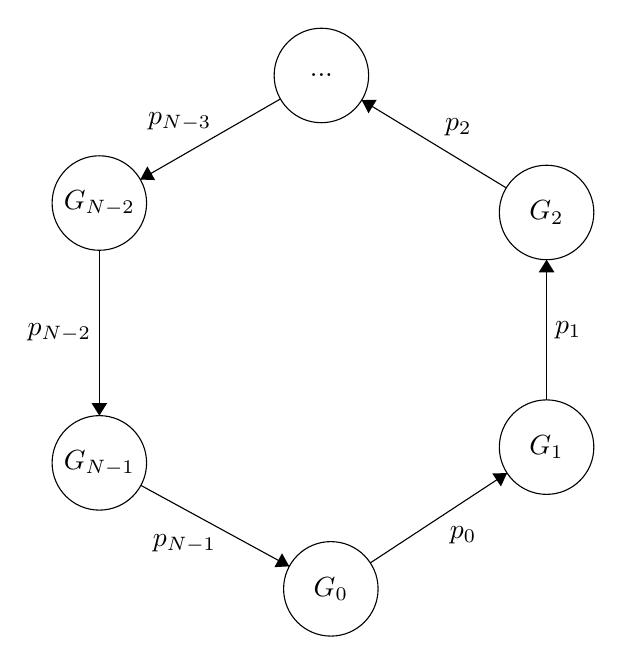
\begin{tikzpicture}[scale=0.2]
		\tikzstyle{every node}+=[inner sep=0pt]
		\draw [black] (38.2,-44.1) circle (3);
		\draw (38.2,-44.1) node {$G_0$};
		\draw [black] (51.9,-35.1) circle (3);
		\draw (51.9,-35.1) node {$G_1$};
		\draw [black] (23.5,-36.1) circle (3);
		\draw (23.5,-36.1) node {$G_{N-1}$};
		\draw [black] (51.9,-20.2) circle (3);
		\draw (51.9,-20.2) node {$G_2$};
		\draw [black] (23.5,-19.6) circle (3);
		\draw (23.5,-19.6) node {$G_{N-2}$};
		\draw [black] (37.6,-11.5) circle (3);
		\draw (37.6,-11.5) node {$...$};
		\draw [black] (40.71,-42.45) -- (49.39,-36.75);
		\fill [black] (49.39,-36.75) -- (48.45,-36.77) -- (49,-37.6);
		\draw (46.6,-40.1) node [below] {$p_0$};
		\draw [black] (26.14,-37.53) -- (35.56,-42.67);
		\fill [black] (35.56,-42.67) -- (35.1,-41.84) -- (34.62,-42.72);
		\draw (28.91,-40.6) node [below] {$p_{N-1}$};
		\draw [black] (23.5,-22.6) -- (23.5,-33.1);
		\fill [black] (23.5,-33.1) -- (24,-32.3) -- (23,-32.3);
		\draw (23,-27.85) node [left] {$p_{N-2}$};
		\draw [black] (51.9,-32.1) -- (51.9,-23.2);
		\fill [black] (51.9,-23.2) -- (51.4,-24) -- (52.4,-24);
		\draw (52.4,-27.65) node [right] {$p_1$};
		\draw [black] (49.34,-18.64) -- (40.16,-13.06);
		\fill [black] (40.16,-13.06) -- (40.59,-13.9) -- (41.11,-13.05);
		\draw (46.3,-15.35) node [above] {$p_2$};
		\draw [black] (35,-12.99) -- (26.1,-18.11);
		\fill [black] (26.1,-18.11) -- (27.04,-18.14) -- (26.55,-17.27);
		\draw (28.6,-15.05) node [above] {$p_{N-3}$};
		\end{tikzpicture}
	}
	\end{tabular}
\caption{Modele gry. G w okręgu - gracz, strzałka z p - prawdopodobieństwo zagrania w celu nawiązania koalicji z graczem, na którego wskazuje strzałka}
\label{fig:modele}
\end{figure}
%---------------------------------------------------------------------------------------------------------------------------------------------------------------------

\section{Równania standardowe}
\label{sec:r_stand}
Pomysł na równania standardowe został zaczerpnięty ze wzoru na siłę w polu potencjału.
\begin{equation}\label{eq:fiz_stand}
\overrightarrow{F}(\overrightarrow{r})=-\nabla \varphi (\overrightarrow{r})
\end{equation}
Z tym że żądana jest maksymalizacja, a nie minimalizacja odpowiednika energii potencjalnej. Z tego powodu należy zmienić znak. Co przekłada się na ogólny wzór, gdzie $\beta$ jest zmienną funkcji W:
\begin{equation}\label{eq:basic_stand}
W_\beta = \frac{\delta W}{\delta \beta}
\end{equation}
W tym typie równań celem będzie maksymalizacja zysku( zyskiem jest prawdopodobieństwo ) w czasie. Wyprowadzenie będzie przeprowadzone dla $G_0$, przy założeniu gry o pełnej informacji. Pozostałe dwa równania można wyprowadzić analogicznie. Niech $x=p_0$, $y=p_1$, $z=p_2$. Wypłata dla $G_0$ dana jest przez:
\begin{equation}\label{eq:wypl_stand}
W = \underbrace{x(1-y)}_{\text{wypłata sojuszu $G_0$ z $G_1$}} + \overbrace{(1-x)z}^{\text{wypłata sojuszu $G_0$ z $G_2$}} \\
\end{equation}
W równaniu \ref{eq:basic_stand} podstawiamy $x$ jako $\beta$.
\begin{align*}
W_x = \frac{\delta W}{\delta x} = 1-y-z
\end{align*}
Iloraz różnicowy na zmianę wypłaty od czasu daje:
\begin{align}\label{eq:dynam_stand}
W_x(t) &= \frac{p_0(t+\Delta t)-p_0(t)}{\Delta t} \nonumber\\
W_x(t) \Delta t &= p_0(t+\Delta t)-p_0(t) = \Delta p_0 \nonumber\\
\Delta p_0 &= \Delta t (1-y-z)
\end{align}
W dalszej części będzie stosowane oznaczenie $\alpha = \Delta t$. Równanie wygląda obiecująco, gdyż człon $1 - y$ jest prawdopodobieństwem zagrania $G_1$ aby zawiązać sojusz z $G_0$. Podobnie $-z$ prowadzi do sojuszu $G_2$ z $G_0$.

W przypadku gry o niepełnej informacji należy zmodyfikować równanie \ref{eq:dynam_stand}. Opis użytych parametrów można znaleźć w podrozdziale \ref{sec:model}.
\begin{equation} \label{eq:stand}
\Delta p_i = \alpha \cdot (1 - \frac{n_{i+1}}{l_p} - \frac{n_{i-1}}{l_p})
\end{equation}

%---------------------------------------------------------------------------------------------------------------------------------------------------------------------

\section{Równania replikatorów}
\label{sec:r_repli}
Model dynamiki replikatorów jest najbardziej znanym różniczkowym modelem teorii gier ewolucyjnych \cite{Now06}\cite{Hof98}, przez co może stanowić dobry wybór do sterowania zachowaniem graczy. Tak jak poprzednio przyjmijmy prawdopodobieństwa $x=p_0$, $y=p_0$ oraz $z=p_0$ pamiętając, że prawdopodobieństwa przeciwników w symulacji są szacowane. Podstawowy wzór równania replikatorów wygląda następująco:
\begin{equation}
\dot{x} = x \cdot ( W_x - \overline{W})
\end{equation}
Gdzie $\dot{x}$ jest tempem zmiany udziału strategi $x$, $W_x$ jest średnią wypłatą dla strategii $x$ (prawdopodobieństw strategii $x$), natomiast $\overline{W}$ jest średnią wypłatą co daje:
\begin{gather*}
\dot{x} = x \cdot ( \overbrace{(1-y)}^{W_x} - \overbrace{(x(1-y) + (1-x)z)}^{\overline{W}}) \\
\Downarrow \\
\dot{x} = x \cdot (1-x) \cdot (1-y-z)
\end{gather*}
Iloraz różnicowy zmiany wypłaty od czasu ponownie wyznaczy $\Delta p_0$:
\begin{align*}
\dot{x}(t) &= \frac{p_0(t+\Delta t)-p_0(t)}{\Delta t} \\
\dot{x}(t) \Delta t &= p_0(t+\Delta t)-p_0(t) = \Delta p_0 \\
\Delta p_0 &= \dot{x}(t) \Delta t
\end{align*} 
W dalszej części tej pracy $\alpha=\Delta t$. Co dla gry 3-osobowej generuje równania:
\begin{align} \label{eq:repli}
\Delta p_0 = \alpha p_0 \cdot (1 - p_0) \cdot (1 - \frac{n_1}{l_p} - \frac{n_2}{l_p}) \nonumber \\
\Delta p_1 = \alpha p_1 \cdot (1 - p_1) \cdot (1 - \frac{n_2}{l_p} - \frac{n_0}{l_p}) \\
\Delta p_2 = \alpha p_2 \cdot (1 - p_2) \cdot (1 - \frac{n_0}{l_p} - \frac{n_1}{l_p}) \nonumber
\end{align} 

%---------------------------------------------------------------------------------------------------------------------------------------------------------------------

\section{Ograniczenie prawdopodobieństwa}
\label{sec:ograniczenie}
Wszystkie zmiany prawdopodobieństwa muszą zostać poddane funkcji ograniczającej.
\begin{equation} \label{eq:ograniczenie}
p_i = ogr( p_i + \Delta p_i)
\end{equation}
W przeciwnym razie równania z poprzednich podrozdziałów mogą wyjść poza przedział $<0,1>$. Każde nowo obliczone prawdopodobieństwo podawane jest jako parametr do funkcji $ogr$, a dopiero jej rezultat jest przypisywany poszczególnym prawdopodobieństwom graczy. Funkcja używana aby zapewnić pozostanie prawdopodobieństwa w dziedzinie wygląda następująco:
\begin{displaymath}
ogr(p_i) = \left\{
\begin{array}{ll}
1 & \text{jeżeli } p_i > 1 \\
p_i & \text{jeżeli } 1 \geq p_i \geq 0 \\
0 & \text{jeżeli } p_i < 0
\end{array} 
\right.
\end{displaymath}
Wyjaśnienia wymaga wartość $\alpha$, która została przyjęta jako $0.1$. Jest to wartość przyjęta arbitralnie aby spowolnić rozgrywkę oraz umożliwić łatwiejszą zmianę koalicji. 

%---------------------------------------------------------------------------------------------------------------------------------------------------------------------

\section{Ograniczenie prawdopodobieństwa - przykłady}
\label{sec:ograniczenie_przyk}
Najpierw przeanalizowane zostaną równania standardowe dla gry 3-osobowej o prawdopodobieństwie początkowym $\frac{1}{2}$ i $\alpha = 1$. Gdzie $N$ oznacza zagranie $G_i$ mające na celu zawiązanie sojuszu z $G_{i+1}$, a $P$ ilość zagranie$G_i$ mające na celu zawiązanie sojuszu z $G_{i-1}$.
\begin{align*}
G_0 = N, G_1 = P, G_2 = N && G_0 = N, G_1 = P, G_2 = P\\
\left\{
\begin{array}{cc}
\Delta p_0 = (1 - 0 - 1) =  0 & p_0=\frac{1}{2}\\
\Delta p_1 = (1 - 1 - 1) =  -1 & p_1= 0\\
\Delta p_2 = (1 - 1 - 0) =  0 & p_2=\frac{1}{2}\\
\end{array} 
\right. &&
\left\{
\begin{array}{cc}
\Delta p_0 = (1 - 0 - \frac{1}{2}) =  0 & p_0=\frac{3}{4}\\
\Delta p_1 = (1 - \frac{1}{2} - 1) =  -\frac{1}{2} & p_1= 0\\
\Delta p_2 = (1 - 0 - \frac{1}{2}) =  \frac{1}{2} & p_2=\frac{3}{4}\\
\end{array}
\right.
\end{align*}
Schemat przedstawia dwie osobne tury: po lewej pierwszą, a po prawej drugą. Parametr $\alpha=1$ powoduje szybkie zawiązanie mocnych koalicji, których przerwanie staje się mało prawdopodobne, co może praktycznie uniemożliwiać jakiekolwiek zmiany sojuszy.

%										REPLIKATORY
Wartym rozważenia jest czy w równaniach replikatorów potrzebna będzie $\alpha < 1$, skoro posiadają one człon postaci $x(1-x)$ gasnący na krańcach przedziału prawdopodobieństwa. Założenia zostały oparte na poprzednim przykładzie.
\begin{gather*}
G_0 = N, G_1 = P, G_2 = N \\
\left\{
\begin{array}{ll}
\Delta p_0 = \frac{1}{2} \cdot (1 - \frac{1}{2}) \cdot (1 - 0 - 1) =  0 & p_0=\frac{1}{2}\\
\Delta p_1 = \frac{1}{2} \cdot (1 - \frac{1}{2}) \cdot (1 - 1 - 1) =  0 & p_1= \frac{1}{4}\\
\Delta p_2 = \frac{1}{2} \cdot (1 - \frac{1}{2}) \cdot (1 - 0 - 1) =  0 & p_2=\frac{1}{2}\\
\end{array} 
\right.
\\
G_0 = N, G_1 = P, G_2 = P \\
\left\{
\begin{array}{ll}
\Delta p_0 = \frac{1}{2} \cdot (1 - \frac{1}{2}) \cdot (1 - 0 - \frac{1}{2}) = \frac{1}{8} & p_0=\frac{5}{8}\\
\Delta p_1 = \frac{1}{4} \cdot (1 - \frac{1}{4}) \cdot (1 - \frac{1}{2} - 1) = -\frac{1}{32} & p_1= \frac{7}{32}\\
\Delta p_2 = \frac{1}{2} \cdot (1 - \frac{1}{2}) \cdot (1 - 0 - \frac{1}{2}) = \frac{1}{8}  & p_2=\frac{5}{8}\\
\end{array}
\right.
\end{gather*}
Jak widać najszybsza zmiana zachodzi dla pierwszego gracza, który traci 25\% z prawdopodobieństwa sojuszu z graczem o wyższym indeksie. W kolejnej partii nie widzimy już tak dużych zmian. Należy odpowiedzieć na pytanie czy jest to na tyle dużo, aby zastosować $\alpha$ taką jak w równaniach standardowych. Powinno się poruszyć dwie kwestie. Dynamika prawdopodobieństwa jest akceptowalna(wynosi do 10\%), ale tylko dla prawdopodobieństw które oddalają się od środka przedziału, a grę rozpoczynamy właśnie w nim. Drugą sprawą jest porównanie obu równań. Porównanie wyników, o różnym kroku czasowym nie jest najłatwiejszą rzeczą do opisania.

%                                                   BRAK WSPÓŁPRACY

Omówiony teraz zostanie szczególny przypadek, gdy w dwóch osobnych grach żadna para graczy nie nawiązała koalicji. Użyte będą równania standardowe, prawdopodobieństwo początkowe $\frac{1}{2}$ oraz $\alpha = 1$.

\begin{align*}
G_0 = N, G_1 = N, G_2 = N && G_0 = P, G_1 = P, G_2 = P \\
\left\{
\begin{array}{ll}
\Delta p_0 = (1 - 1 - 1) =  -1 & p_0=0\\
\Delta p_1 = (1 - 1 - 1) =  -1 & p_1= 0\\
\Delta p_2 = (1 - 1 - 1) =  -1 & p_2=0\\
\end{array} 
\right. &&
\left\{
\begin{array}{ll}
\Delta p_0 = (1 - 0 - 0) =  1 & p_0= 1\\
\Delta p_1 = (1 - 0 - 0) =  1 & p_1= 1\\
\Delta p_2 = (1 - 0 - 0) =  1 & p_2= 1\\
\end{array}
\right.
\end{align*}
Przypadek ten pokazuje skutki braku ograniczenia kroku czasowego. Następny ruch jest z góry znany, każdy z graczy wykona ruch przeciwny do poprzedniego co daje w obu grach:
\begin{align*}
\left\{
\begin{array}{l}
\Delta p_0 = (1 - \frac{1}{2} - \frac{1}{2}) =  0 \\
\Delta p_1 = (1 - \frac{1}{2} - \frac{1}{2}) =  0 \\
\Delta p_2 = (1 - \frac{1}{2} - \frac{1}{2}) =  0 \\
\end{array} 
\right.
\end{align*}
Brak zmian prawdopodobieństw, gracze dokonują wyboru jak poprzednio.
\begin{align*}
G_0 = P, G_1 = P, G_2 = P && G_0 = N, G_1 = N, G_2 = N \\
\left\{
\begin{array}{ll}
\Delta p_0 = (1 - \frac{1}{3} - \frac{1}{3}) =  \frac{1}{3} & p_0= \frac{1}{3}\\
\Delta p_1 = (1 - \frac{1}{3} - \frac{1}{3}) =  \frac{1}{3} & p_1= \frac{1}{3}\\
\Delta p_2 = (1 - \frac{1}{3} - \frac{1}{3}) =  \frac{1}{3} & p_2= \frac{1}{3}\\
\end{array} 
\right. &&
\left\{
\begin{array}{ll}
\Delta p_0 = (1 - \frac{2}{3} - \frac{2}{3}) =  -\frac{1}{3} & p_0= \frac{2}{3}\\
\Delta p_1 = (1 - \frac{2}{3} - \frac{2}{3}) =  -\frac{1}{3} & p_1= \frac{2}{3}\\
\Delta p_2 = (1 - \frac{2}{3} - \frac{2}{3}) =  -\frac{1}{3} & p_2= \frac{2}{3}\\
\end{array}
\right.
\end{align*}
Nie jest to powrót do punktu wyjścia, w którym wyjściowym prawdopodobieństwem jest $\frac{1}{3}$ dla gry przedstawionej po lewej stronie i $\frac{2}{3}$ dla gry po prawej. W pamięci każdego z graczy jest liczba rozegranych partii ze swoimi rywalami co będzie prowadziło do niekoniecznie oczywistych zachowań.
Od teraz dokonywany wybór będzie tym o większym prawdopodobieństwie.

\begin{align*}
G_0 = P, G_1 = P, G_2 = P && G_0 = N, G_1 = N, G_2 = N \\
\left\{
\begin{array}{cc}
\Delta p_0 = (1 - \frac{1}{4} - \frac{1}{4}) =  \frac{1}{2} & p_0= \frac{5}{6}\\
\Delta p_1 = (1 - \frac{1}{4} - \frac{1}{4}) =  \frac{1}{2} & p_1= \frac{5}{6}\\
\Delta p_2 = (1 - \frac{1}{4} - \frac{1}{4}) =  \frac{1}{2} & p_2= \frac{5}{6}\\
\end{array} 
\right. &&
\left\{
\begin{array}{cc}
\Delta p_0 = (1 - \frac{2}{5} - \frac{2}{5}) =  -\frac{1}{2} & p_0= \frac{1}{6}\\
\Delta p_1 = (1 - \frac{2}{5} - \frac{2}{5}) =  -\frac{1}{2} & p_1= \frac{1}{6}\\
\Delta p_2 = (1 - \frac{2}{5} - \frac{2}{5}) =  -\frac{1}{2} & p_2= \frac{1}{6}\\
\end{array}
\right.
\end{align*}
Obserwowana jest zmiana zachowania graczy spowodowana częstością gier przeciwników. Sytuacja takiej fluktuacji może się powtarzać. Dysponując odpowiednio dużą grupą instancji gry oraz dostatecznie długą rozgrywką możliwe byłoby zaobserwowanie funkcji prawdopodobieństwa od czasu (równą dla wszystkich graczy instancji) w kształcie sinusoidy o rosnącym okresie.
Sytuacja taka nie jest pożądana, co stanowi dodatkowy argument za użyciem $\alpha < 1$ skutecznie niwelującego wystąpienie takich sytuacji.

\section{Rozwiązanie stacjonarne równań standardowych}
\label{sec:stab_stand}
Celem tego podrozdziału jest znalezienie rozwiązań stacjonarnych dla równań standardowych, czyli sytuacji w których układ dla długiego czasu dąży do punktu stałego. Do ustalenia punktów stałych potrzebny jest zanik dynamiki $\Delta p_i = 0$. Krok czasowy zostanie pominięty, gdyż nie daje wkładu do obliczeń. Należy rozwiązać układ równań, gdzie przyjęte jest $x=p_0$, $y=p_1$, $z=p_2$:
\begin{equation}
\left\{
\begin{array}{c}
1 - y - z = 0 \\
1 - x - z = 0 \\
1 - x - y = 0
\end{array}
\right. \Rightarrow p_0 = p_1 = p_2 = \frac{1}{2}
\end{equation}
Z czego wynika że gra startująca w punkcie $(\frac{1}{2},\frac{1}{2},\frac{1}{2})$ nie powinna z niego wyjść. Byłoby tak gdyby prawdopodobieństwa użyte w równaniu były faktycznymi prawdopodobieństwami $p_i$, są one natomiast jedynie obserwacją zachowania pozostałych graczy. Są ono dane jako $\frac{n_j}{l_p}$. Użycie prawdopodobieństw obserwowanych umożliwia opuszczenie punktu stałego.
\section{Stabilność równań replikatorów}
\label{sec:stab_repl}
Stabilność równań replikatorów \cite{Sss} wymaga dążenia do stałych wartości, gdy $t\Rightarrow \infty$. Do analizy zostanie przyjęty układ równań:
\begin{align}\label{eq:stab_uklad_analiza}
\dot{x} &= f(x,y,z) = \Delta p_0 = x(1-x)(1-y-z)\nonumber\\
\dot{y} &= g(x,y,z) = \Delta p_1 = y(1-y)(1-x-z)\\
\dot{z} &= h(x,y,z) = \Delta p_2 = z(1-z)(1-x-y)\nonumber
\end{align}

Punkty stałe są to punkty, z których układ nie wyjdzie bez zewnętrznego czynnika. Do znalezienia punktów stałych wymagane jest zanikanie pochodnych. Prowadzi to do układu równań.
\begin{align}
\begin{array}{ccc}
\dot{x} = 0, & \dot{y} = 0, & \dot{z} = 0
\end{array}
\end{align}

Z powyższych równań otrzymujemy punkty stałe $(x^*_i, y^*_i, z^*_i)$, które zostały ponumerowane przy pomocy indeksu $i$.
\begin{align}
(x^*_i, y^*_i, z^*_i) = \left\{
\begin{array}{ll}
(0,0,0)  & i=0 \\
(\frac{1}{2},\frac{1}{2},\frac{1}{2}) & i=1 \\
(1,1,1) & i=2 \\
P_3 \{0,1,\xi \} & i=3 \text{, permutacja gdzie }\xi \in <0,1>\\ 
\end{array}
\right.
\end{align}

Znajomość punktów stałych narzuca pytanie co do ich stabilności. Układ znajdujący się w pobliżu punktu stabilnego powinien zawsze do niego dążyć. Podczas analizy stabilności będą uwzględnione wszystkie powyższe punkty stałe, przy czym w ostatniej sytuacji będzie uwzględniony tylko przypadek $(0,1,\xi)$, ze względu na ich symetrię.

Stosując metodę linearyzacji tworzymy funkcje, które powinny osiągać 0 w punktach stabilnych.
\begin{align}\label{eq:nowe_f}
X(t)=x(t)-x^* \nonumber\\
Y(t)=y(t)-y^* \\
Z(t)=z(t)-z^* \nonumber
\end{align}

Zróżniczkowanie funkcji \ref{eq:nowe_f} i rozwinięcie w szereg Taylora do pierwszej pochodnej dają:
\begin{align}
\dot{X}(t)=\dot{x}(t)-\dot{x}^* &=\dot{x}(t)=f(x(t),y(t),z(t))=f(x^*+X(t),y^*+Y(t),z^*+Z(t))= \nonumber\\
&=f(x^*,y^*,z^*)+\frac{\delta f(x^*,y^*,z^*)}{\delta x}X+\frac{\delta f(x^*,y^*,z^*)}{\delta y}Y+\frac{\delta f(x^*,y^*,z^*)}{\delta z}Z \nonumber\\
\dot{Y}(t)=\dot{y}(t)-\dot{y}^* &=\dot{y}(t)=g(x(t),y(t),z(t))=g(x^*+X(t),y^*+Y(t),z^*+Z(t))=\\
&=g(x^*,y^*,z^*)+\frac{\delta g(x^*,y^*,z^*)}{\delta x}X+\frac{\delta g(x^*,y^*,z^*)}{\delta y}Y+\frac{\delta f(x^*,y^*,z^*)}{\delta z}Z \nonumber\\
\dot{Z}(t)=\dot{z}(t)-\dot{z}^* &=\dot{z}(t)=h(x(t),y(t),z(t))=h(x^*+X(t),y^*+Y(t),z^*+Z(t))=\nonumber\\
&=f(x^*,y^*,z^*)+\frac{\delta h(x^*,y^*,z^*)}{\delta x}X+\frac{\delta h(x^*,y^*,z^*)}{\delta y}Y+\frac{\delta h(x^*,y^*,z^*)}{\delta z}Z\nonumber
\end{align}

Wiadomo że w punktach stacjonarnych $\dot{x}= \dot{y} =\dot{z} =0$, na podstawie czego można przyjąć, że $f(x^*,y^*,z^*)=g(x^*,y^*,z^*)=h(x^*,y^*,z^*)=0$. Pierwszy i ostatni człon powyższych równań dają układ równań.
\begin{align}
\begin{array}{c}
\dot{X}=a_{11}X+a_{12}Y+a_{13}Z \\
\dot{Y}=a_{21}X+a_{22}Y+a_{23}Z \\
\dot{Z}=a_{31}X+a_{32}Y+a_{33}Z
\end{array}
\end{align}

Macierz współczynników można zapisać jako macierz Jacobiego.
\begin{align*}
J_i= \left. \left[
\begin{array}{ccc}
\frac{\delta \dot{x}}{\delta x} & \frac{\delta \dot{x}}{\delta y} & \frac{\delta \dot{x}}{\delta z} \\
\frac{\delta \dot{y}}{\delta x} & \frac{\delta \dot{y}}{\delta y} & \frac{\delta \dot{y}}{\delta y} \\
\frac{\delta \dot{z}}{\delta x} & \frac{\delta \dot{z}}{\delta y} & \frac{\delta \dot{z}}{\delta x}
\end{array}
\right]
\right|_{
	\begin{array}{c}
		x=x^*_i\\
		y=y^*_i\\
		z=z^*_i	
	\end{array}	
}
= \left[
\begin{array}{ccc}
a_{11} & a_{12} & a_{13} \\
a_{21} & a_{22} & a_{23} \\
a_{31} & a_{32} & a_{33}
\end{array}
\right] \text{dla }i\text{-tego punktu stałego}
\end{align*}

Pochodne cząstkowe:
\begin{align*}
\begin{array}{l}
\frac{\delta \dot{x}}{\delta x} = 1-y-z-2x+2xy+2xz\\
\frac{\delta \dot{x}}{\delta y} = x^2 - x\\
\frac{\delta \dot{x}}{\delta z} = x^2 - x\\
\end{array}
&&
\begin{array}{l}
\frac{\delta \dot{y}}{\delta x} = y^2 - y\\
\frac{\delta \dot{y}}{\delta y} = 1-x-z-2y+2xy+2yz\\
\frac{\delta \dot{y}}{\delta z} = y^2 - y\\
\end{array}
\end{align*}
\begin{align*}
\begin{array}{l}
\frac{\delta \dot{z}}{\delta x} = z^2 - z\\
\frac{\delta \dot{z}}{\delta y} = z^2 - z\\
\frac{\delta \dot{z}}{\delta z} = 1-x-y-2z+2xz+2yz\\
\end{array}
\end{align*}

Do rozwiązania jest układ równań dany w zapisie macierzowym.
\begin{align}\label{eq:uklad_rown_stab}
\left[ \begin{array}{c}
\dot{X} \\
\dot{Y} \\
\dot{Z}
\end{array}
\right] = 
\left[
\begin{array}{ccc}
a_{11} & a_{12} & a_{13} \\
a_{21} & a_{22} & a_{23} \\
a_{31} & a_{32} & a_{33}
\end{array}
\right] \cdot 
\left[
\begin{array}{c}
X\\
Y\\
Z
\end{array}
\right]
\end{align}

W tym celu wyznaczymy wartości własne.
\begin{align}
J_{i,\lambda} = J_i - \lambda I = 
\left|
\begin{array}{ccc}
\frac{\delta \dot{x}}{\delta x}-\lambda & \frac{\delta \dot{x}}{\delta y} & \frac{\delta \dot{x}}{\delta z} \\
\frac{\delta \dot{y}}{\delta x} & \frac{\delta \dot{y}}{\delta y}-\lambda & \frac{\delta \dot{y}}{\delta z} \\
\frac{\delta \dot{z}}{\delta x} & \frac{\delta \dot{z}}{\delta y} & \frac{\delta \dot{z}}{\delta z}-\lambda
\end{array}
\right| = 0
\end{align}
\begin{equation*}
\lambda =
\left\{
\begin{array}{l}
\lambda_0 \in \{1,1,1\}\\
\lambda_1 \in \{-\frac{1}{2}, \frac{1}{4}, \frac{1}{4}\}\\
\lambda_2 \in \{1,1,1\}\\
\lambda_3 \in \{0,-z, z-1\}
\end{array}
\right.
\end{equation*}

W rozwiązaniu ogólnym układu \ref{eq:uklad_rown_stab} dla punktu stałego $(x^*_i, y^*_i, z^*_i)$ wartości własne odpowiadające zmiennym $x$, $y$, $z$ są odpowiednio $\alpha_i$, $\beta_i$, $\gamma_i$. Wektorami własnymi dla poszczególnych wartości własnych są $V_i$, natomiast $C_i$ są współczynnikami rozwiązania jednorodnego układu równań różniczkowych. 
\begin{align}\label{eq:rozw_ur}
\left[ \begin{array}{c}
X(t)\\
Y(t)\\
Z(t)
\end{array}
\right] = C_{\alpha_i} V_{\alpha_i} e^{\alpha_it} + C_{\beta_i} V_{\beta_i} e^{\beta_it} + C_{\gamma_i} V_{\gamma_i} e^{\gamma_it}
\end{align}

Aby punkt był stabilny funkcje muszą dążyć w czasie do zera.
\begin{align}
\begin{array}{ccc}
\displaystyle\lim_{t \to \infty} X(t)=0 & \displaystyle\lim_{t \to \infty} Y(t)=0 & \displaystyle\lim_{t \to \infty} Z(t)=0
\end{array}
\end{align}

Aby eksponenta malała musi posiadać ujemny wykładnik, z czego wynika że warunkiem stabilności jest:
\begin{equation}\label{eq:war_stab}
Re(\lambda_a)<0 \wedge Re(\lambda_b)<0 \wedge Re(\lambda_c)<0
\end{equation}

Warunek \ref{eq:war_stab} eliminuje wszystkie lambdy poza $\lambda_3$. Pokazuje to że punkty o kombinacji $(0,1,\xi)$ są marginalnie stabilne. Analiza nie wskazuje że są stabilne, lecz temu też nie przeczy. W celu analitycznego określenia stabilności należałoby rozwiązać układ równań \ref{eq:rozw_ur}.

\begin{wraptable}{rh}{0.35\textwidth}
    \centering
    \caption{Stabilność na krawędzi sześcianu}
\label{tab:krawedz_prawd}
\begin{tabular}{c|c|c|c}
x & y & 1-x-y & $\dot{z}$       \\ \hline 
0 & 0 & 1     & $z \cdot (1-z)$  \\
0 & 1 & 0     & 0                \\
1 & 0 & 0     & 0                \\
1 & 1 & -1    & $-z \cdot (1-z)$
\end{tabular}
\end{wraptable}

Mając wiedzę że symulacja rozpoczyna się z punktu $(\frac{1}{2},\frac{1}{2},\frac{1}{2})$ znamy wartość $X(0)$, $Y(0)$, $Z(0)$ z czego można wyliczyć $C_i$. Jeśli będą one równe 0 dla wartości własnych równych 0 punkt jest stabilny, w przeciwny wypadku nie jest stabilny. Jest to nieelegancka i mozolna metoda.
 
Ponieważ analiza matematyczna nie przyniosła jednoznacznej odpowiedzi co do stabilności punktów $(0,1,\xi)$, można spróbować przeanalizować równanie $\dot{z}$ - układ \ref{eq:stab_uklad_analiza}, dla sytuacji gdy $p_i$ dwóch z graczy dojdą do granicy prawdopodobieństwa. Warto przeanalizować wszystkie przypadki pomimo, że dla omawianych punktów tylko wiersz drugi i trzeci ma znaczenie. Celem poniższej analizy jest sprawdzenie czy wspomniane punkty są stabilne po ich osiągnięciu.
W pierwszym wierszu tabelki \ref{tab:krawedz_prawd} widać, że $G_0$ dąży do zawarcia sojuszu z $G_2$, natomiast $G_1$ gra aby osiągnąć sojusz z $G_0$. W tej sytuacji prawdopodobieństwo $z$, że gracz $G_2$ zawiąże koalicję z $G_0$ będzie rosło. W kolejnych dwóch wierszach są stany ustalone. W wierszu drugim zmiana $\dot{z}$ nie ma znaczenia gdyż gracze $G_0$ oraz $G_1$ są w wyłącznej koalicji z $G_2$. Wiersz trzeci pokazuje przeciwną sytuację, w której jakakolwiek zmiana $\dot{z}$ nie wniesie nic do gry ze względu na trwały sojusz między $G_0$ a $G_1$. Ostatni wiersz pokazuje przypadek symetryczny do pierwszego, z tym że jedynym możliwym sojusznikiem dla $G_2$ jest $G_1$. Oczywiście omawiany teraz przykład do osiągnięcia stabilności wymagałby braku zmian decyzji pozostałych graczy. Musieli by oni znać realne prawdopodobieństwo przeciwników.